% *******************************************************************************
% * Copyright (c) 2007 by Elexis
% * All rights reserved. This document and the accompanying materials
% * are made available under the terms of the Eclipse Public License v1.0
% * which accompanies this distribution, and is available at
% * http://www.eclipse.org/legal/epl-v10.html
% *
% *  $Id: icpc-plugin.tex 1951 2007-02-26 09:34:52Z rgw_ch $
% *******************************************************************************
% !Mode:: "TeX:UTF-8" (encoding info for WinEdt)

\section{ICPC}
Das Plugin ICPC bindet einerseits den \textit{International Code for Primary Care} Version 2 in Elexis ein, ermöglicht einerseits auch unabhängig davon die strukturierte problemorientierte KG-Führung.
\index{problemorientierte KG}
\index{Problem}
\subsection{Problemliste}
\begin{wrapfigure}{r}{6cm}
  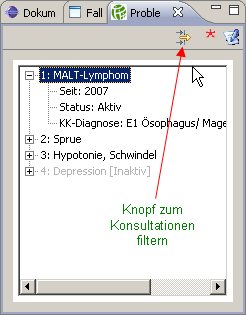
\includegraphics{images/problemliste1}
  \caption{Problemliste}\label{fig:problemliste}
\end{wrapfigure}

Die Problemliste (Abb. \ref{fig:problemliste}) erlaubt Ihnen, Probleme (auch bezeichnet als Krankheitsepisoden) als Freitext einzugeben und ihnen eine Nummer zuzuordnen. Bei der Darstellung werden sie automatisch anhand dieser Nummern sortiert. Wenn Sie also einem Problem eine tiefere Priorität zuordnen wollen, genügt es, ihm eine niedrigere Nummer zu geben. Wenn Sie ein Problem zum Unterproblem eines anderen Problems machen wollen, können Sie eine Nummer mit einem Punkt angeben: Problem 2.1 wird automatisch dem Problem 2 zugeordnet und zwischen 2 und 3 angezeigt.

Um ein neues Problem einzugeben, klicken Sie auf das Stern-Symbol in der Titelzeile der View; um es zu löschen klicken Sie es mit der rechten Maustaste an und wählen \textit{löschen}. Um die Eigenschaften eines existierenden Problemeintrags zu bearbeiten, klicken Sie auf das Bearbeiten-Symbol.

Ein Problem kann verschiedene Eigenschaften haben, beispielsweise ein Beginndatum, einen Status (aktiv oder inaktiv) und eine zugeordnete KK-Diagnose. Diese Eigenschaften werden angezeigt, wenn Sie das kleine plus-Zeichen links neben dem Titel anklicken. Um ein Problem als aktiv oder inaktiv zu markieren. klicken Sie es mit der rechten Maustaste an und wählen die entsprechende Einstellung im Kontextmenü.

Um einem Problem eine KK-Diagnose zuzuordnen (das ist die Diagnose, die später auf der Rechnung erscheinen wird), können Sie eine solche Diagnose einfach aus einer Diagnoseliste, etwa aus dem Behandlungsfenster etc. auf das entsprechende Problem ziehen.

\begin{figure}[ht]
    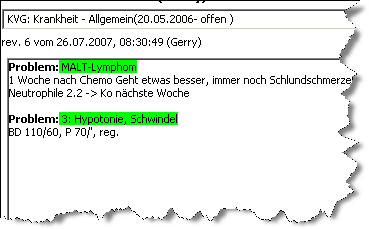
\includegraphics{images/problemliste2}
    \caption{Problem in Konsultationstext}
    \label{fig:problemliste2}
\end{figure}
Um ein Problem in einer Konsultation explizit zu behandeln, ziehen Sie es mit der Maus aus der Problemliste in Ihr Konsultationsfenster (Abb. \ref{fig:problemliste2}).

Wenn Sie konsequent mit der Problemliste arbeiten, erhalten Sie einen zusätzlichen Nutzen: Wenn Sie den Filtern-Knopf im Problemliste-Fenster einrasten (Abb. \ref{fig:problemliste}), dann werden in der Konsultationen-View (\ref{view:konsultationen}; s. \pageref{view:konsultationen} ff.) automatisch immer nur diejenigen Konsultationen angezeigt, die das gerade ausgewählte Problem behandeln. 
\label{filter:problemliste}
\index{konsultationen!filtern} \index{Filter}Klick auf ein anderes Problem filtert die Konsultationen-Liste jeweils neu. Erneuter Klick auf den Filtern-Knopf löst diesen wieder aus, so dass wieder alle Konsultationen angezeigt werden.

\subsection{Encounter}
Um das ICPC-Plugin voll nutzen zu können, benötigen Sie den ICPC-Code selbst, den Sie leicht importieren können. Aus lizenzrechtlichen Gründen können wir ihn aber nicht direkt beifügen. Erkundigen Sie sich bitte ggf. bei der SGAM, ob und unter welchen Bedingungen Sie den Code beziehen können.
\subsubsection{Idee}
Der Gedanke hinter ICPC ist, dass die Arbeit des family doctors besser abgebildet werden soll, als es mit Codes wie ICD-10 oder Tarmed möglich ist. Es muss möglich sein, auch Alltagsdinge wie \glqq fühlt sich unwohl\grqq oder \glqq hat Angst vor Krebs\grqq zu codieren und Handlungen wie \glqq habe in untersucht, beraten und die Ängste ausgeräumt\grqq zu deklarieren, und auch die Diagnise \glqq ist gesund\grqq muss möglich sein. Wenn man solche Dinge in strukturierter Weise festhält, kann man die Arbeit des Allgemeinarztes viel besser erforschen, vergleichen und quantifizieren, als dies mit anderen Codesystemen möglich ist. Grundversorgerverbände verschiedener Länder haben daher ein erhebliches Interesse, ICPC zur Stärkung ihrer Datenbasis und damit Förderung einer besseren Grundversorger-orientierten Politik einzusetzen (Dass der Code dennoch nicht kostenlos zur Verfügung gestellt wird, ist wohl einer dieser Logik-Loopings, die beim Entwickeln von Realpolitik aus guten Ideen manchmal passieren...)

\subsubsection{Einführung}
Konkret geschieht die Codierung nach ICPC so, dass der Schnittpunkt einer Krankheits-Episode (eines Problems wie im vorherigen Abschnitt geschildert) mit einer Konsultation ein \textit{Encounter} entsteht. Wenn bei einer Konsultation also zwei Probleme behandelt werden, entsthehen genau zwei Encounters, auch wenn der Patient vielleicht 5 Probleme in der Problemliste stehen hat.

Jeder Encounter ist gekennzeichnet durch
\begin{itemize}
\item Einen Grund (reason for encounter, rfe): Wieso kam der Patient? Beispiel: 'Kopfschmerzen'.
\item Eine Beurteilung (Diagnose). Zum Beispiel 'Migräne'.
\item Ein Procedere. Zum Beispiel 'Medikament, Lebensstilberatung'.
\end{itemize}


\section{Sgam-xChange}
Sgam-xChange ist ein Plugin, das den Austausch von beliebigen Daten zwischen elKG-Systemen ermöglicht. Sie können beispielsweise ein Laborblatt oder eine ganze KG aus Ihrem Programm exportieren, verschlüsselt zu einem Kollegen transportieren, der es dann in seine elKG importieren kann - sofern diese ebenfalls xChange-fähig ist.Sgam-xChange ist ein Plugin, das den Austausch von beliebigen Daten zwischen elKG-Systemen ermöglicht. Sie können beispielsweise ein Laborblatt oder eine ganze KG aus Ihrem Programm exportieren, verschlüsselt zu einem Kollegen transportieren, der es dann in seine elKG importieren kann - sofern diese ebenfalls xChange-fähig ist.

xChange ist ein offener Standard, der folgende Elemente beinhaltet:
\begin{itemize}
 \item Transport-Datenformat, damit die beteiligten elKG-Programme die Daten \textit{verstehen} können, die sie intern vermutlich auf ganz unterschiedliche Weise speichern.
\item Transport-Container, welcher eine Verschlüsselungs- und Transfertechnologie definiert, damit diese Daten sicher und vertraulich vom Sender zum Empfänger gelangen.
\end{itemize}
Um es jedem Hersteller von Praxisprogrammen zu ermöglichen, xChange zu implementieren, wurde der Standard bewusst auf die wesentlichsten Elemente limitiert, und er wird jedem Interessenten kostenlos zur Verfügung gestellt, inklusive einer Beispielanwendung, die konkrete Implementationshinweise gibt.

Sgam-xChange entstand im Auftrag und unter Sponsoring der Arbeitsgruppe \href{http://www.sgam.ch/informatics}{Sgam.informatics} , welche auch Ansprechpartner für alle Lizenzfragen ist.

\subsection{Voraussetzungen}


Eine Erläuterung und Beschreibung der technischen Hintergründe finden Sie hier .
 Dieser Artikel beschränkt sich im Folgenden auf die Beschreibung der in Elexis eingebauten Implementation von Sgam.xChange.

Um Daten aus Elexis mittels Sgam.xChange transportieren zu können, benötigen Sie ausser Elexis und dem Sgam.xChange-Plugin (welches standardmässig integriert ist), noch das Verschlüsselungsprogramm \href{http://www.gnupg.org}{GnuPG}.

 GnuPG ist für die meisten wichtigen Betriebssysteme (Windows, Linux, Mac) erhältlich und ist kostenlos. Es ist ein OpenSource-Verschlüsselungssystem, das seit 1999 existiert und weltweit einen ausgezeichneten Ruf geniesst (ist beispielsweise in manchen Ländern verboten, weil es von Geheimdiensten nicht geknackt werden kann). In der Schweiz ist seine Anwendung legal.

\subsection{Installation und Konfiguration}

GPG kann an beliebiger Stelle installiert werden; es muss dann lediglich an Elexis bekanntgemacht werden, wo es liegt. Öffnen Sie dazu im Menü \textit{Datei-Einstellungen} den Reiter \textit{xChange}:

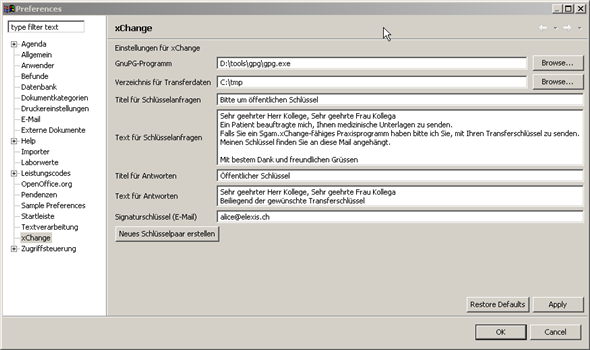
\includegraphics[width=3in]{images/xc1.png}
% xc1.png: 590x350 pixel, 96dpi, 15.61x9.26 cm, bb=0 0 442 262

Folgende Einstellungen können hier vorgenommen werden:
\begin{itemize}
 \item GnuPG-Programm: Den vollständigen Pfad zu gpg.exe
\item Verzeichnis für Transferdaten: Ein existierendes Verzeichnis, in das xChange Dateien zwischenspeichern kann
\item Titel für Schlüsselanfragen: xChange kann automatische Mails generieren, um  den öffentlichen Schlüssel des Austauschpartners anzufordern. Hier können Sie den Titel einsetzen, den eine solche Mail haben soll.
\item Text für Schlüsselanfragen: Hierhin kommt der Text, welcher in eine Schlüsselanforderungs-Mail gesetzt werden soll.
\item Titel für Antworten: Auch für die Beantwortung einer Schlüsselanfrage kann xChange automatisch eine E-Mail generieren. Hierhin kommt der Titel einer solchen Antwort
\item Text für Antworten: Der Textinhalt einer Antwort-Mail
Signaturschlüssel (E-Mail): Hier sollten Sie denjenigen Schlüssel angeben, der standardmässig für xChange verwendet werden soll. Oft wird das sowieso Ihr einziger Schlüssel sein. Geben Sie dabei die E-Mail ein, die mit diesem Schlüssel Verknüpft ist.

\item
\item Neues Schlüsselpaar erstellen: Falls Sie noch keinen GPG-Schlüssel haben, können Sie nach Klick auf diesem Knopf ein Paar erstellen (Ein Schlüsselpaar besteht aus einem mit einem Passwort gesicherten privaten Schlüssel, den Sie zum Signieren und zum Entschlüsseln brauchen, und aus dem dazu passenden öffentlichen Schlüssel, den Sie jedem Interessenten geben können, um damit Nachrichten an Sie verschlüsseln und Signaturen von Ihnen verifizieren zu können)

\end{itemize}

Nach Knopfdruck erscheint dieses Fenster:

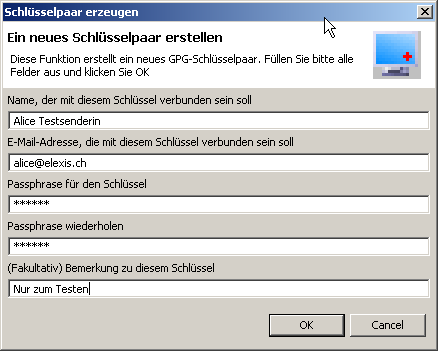
\includegraphics[width=3in]{images/xc2.png}
% xc2.png: 438x351 pixel, 96dpi, 11.59x9.29 cm, bb=0 0 328 263

Die Angaben sind selbsterklärend. xChange wird Ihre Sendungen jeweils mit diesem Schlüssel signieren und wird Sendungen, die an Sie gerichtet sind, mit diesem Schlüssel zu decodieren versuchen.
(Genauere Erklärungen zu den Schlüsseln finden Sie \href{http://www.elexis.ch/jp/index.php?option=content&task=view&id=64}{hier})
\subsection{Eine Krankengeschichte exportieren}
Klicken Sie mit der rechten Maustaste auf den gewünschten Patienteneintrag und wählen Sie \textit{KG Exportieren}

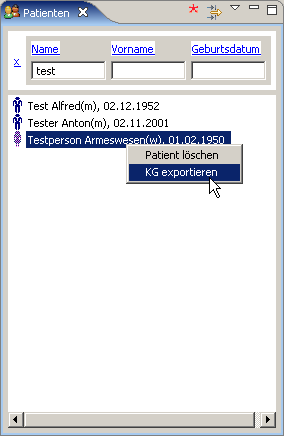
\includegraphics[width=3in]{images/xc3.png}
% xc3.png: 284x436 pixel, 96dpi, 7.51x11.53 cm, bb=0 0 213 327

 Es erscheint folgender Dialog:

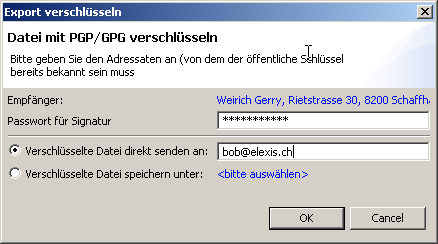
\includegraphics[width=3in]{images/xc4.png}
% xc4.png: 438x244 pixel, 96dpi, 11.59x6.46 cm, bb=0 0 328 183

Nach Klick auf \textit{OK} wird die KG automatisch verschlüsselt und an den Empfänger gesandt, der sie nur mit seinem, oben unter \textit{Empfänger} genannten Schlüssel wieder entschlüsseln kann.

\subsection{Die Empfängerseite}
Auf der Empfängerseite kommt nun die eben abgeschickte E-Mail an:


\includegraphics[width=3in]{images/import1.png}
% import1.png: 644x369 pixel, 72dpi, 22.72x13.02 cm, bb=0 0 644 369

Der Mail-Anhang ist die xChange-Datei.


\includegraphics[width=3in]{images/import2.png}
% import2.png: 540x134 pixel, 72dpi, 19.05x4.73 cm, bb=0 0 540 134

Diese kann gespeichert und direkt nach Elexis eingelesen werden aus dem Menu Datei-Import.

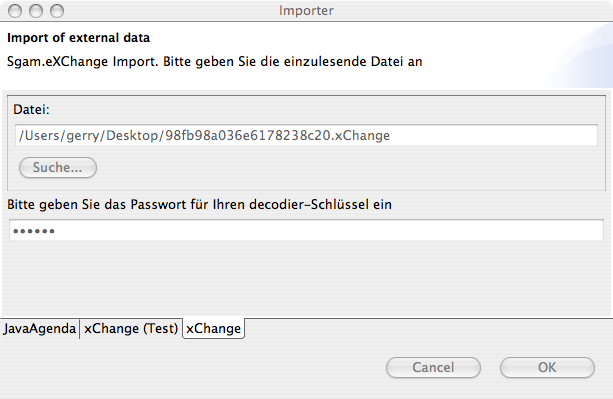
\includegraphics[width=3in]{images/import3.png}
% import3.png: 613x399 pixel, 72dpi, 21.63x14.08 cm, bb=0 0 613 399



Sofern Sie im Besitz des korrekten Schlüssels sind, wird die KG jetzt in Ihrem Programm importiert.

Zum Konzept der Schlüsselverwaltung lesen Sie bitte \href{http://www.elexis.ch/jp/index.php?option=content&task=view&id=64}{hier} mehr Einzelheiten.

\section{Elexis-ebanking-Schweiz}
Einbindung des Schweizer ESR/DTA-Systems zum bargeldlosen Zahlungsverkehr. Dieses Plugin ist Teil der Standard-Distribution. Es hat selbst keine Benutzerfunktionen, muss aber vorhanden sein, wenn andere Plugins diese E-Banking-Funktionen nutzen wollen.
